\chapter{Introduction}
\section{Single-cell RNA sequencing}
Recent advances in single-cell RNA sequencing (scRNA-seq) technologies\cite{Kolodziejczyk2015} have boosted many biological and clinical discoveries at an unprecedented resolution. Previously, sequencing technologies, such as bulk RNA-seq\cite{Emrich2007}, can only provide a gene expression profile of an entire sample containing thousands to millions of cells, revealing an overall state and biological traits of a whole organ or tissue. However, knowledge from a population of cells cannot represent that from an individual cell since biological signals of a minority of cells within a cell pool or slight differences in two cells of the same cell type may fail to be effectively detected\cite{Haque2017}, for example, malignant tumor cells within a tumor mass\cite{Tirosh2016} and individual T cells with highly diverse T cell receptors\cite{Stubbington2016}. To address this issue, scRNA-seq can be used to disentangle single cells from pooled cells, providing cellular heterogeneity that is valuable for many research focuses such as cellular traits, cellular responses to different scenarios and so on. In addition, data generated from scRNA-seq is also beneficial to gene regulatory networks (GRN) inferences in a data-driven way, providing context-specific GRNs which enables us to decipher functional cellular heterogeneity\cite{Haque2017}. Nevertheless, although scRNA-seq fulfills high-resolution transcriptomic analysis, it still has some challenges and limitations, such as drop-out events due to extremely low gene expression\cite{Ran2020}, batch effects between datasets from different measurements\cite{Tran2020} and so on, which complicates scRNA-seq data analysis\cite{Liu2016}. To extract meaningful biological information from high-dimensional noisy scRNA-seq data (i.e., dimensionality reduction), the selected computational method is critical. There are a variety of developed or developing computational methods used for data dimensionality reduction, e.g., for linear algorithms, principal component analysis\cite{Jolliffe2016} (PCA) and non-negative matrix factorization\cite{Quintero2020} (NMF). Compared to linear algorithms, nonlinear algorithms such as deep learning-based models have been proved to be a more advanced technique to learn more complex patterns from noisy transcriptomic data. Specifically, we focused on autoencoder-based models in our work.

\section{Autoencoder-based approaches}
Autoencoders\cite{Hinton2006} (AEs) have emerged as potent tools to tackle many different biological tasks such as dimensionality reduction of data\cite{Wang2018}, cell clustering\cite{Geddes2019} and data denoising\cite{Eraslan2019}. Compared to those methods that are limited by their linear nature (e.g., PCA), AEs are capable of learning more complex nonlinear patterns in single-cell transcriptomes. Generally, AEs consist of two parts: An encoder which can learn a nonlinear transformation projecting data from the high-dimensional input space to the lower-dimensional latent space (i.e., the representations of the input data) and a decoder which also learns a nonlinear transformation projecting the representations from the low-dimensional latent space back to the original high-dimensional input space\cite{Kleut2020} (Fig.\ref{fig:graphical_abstract_AE}). To optimize the quality of the information that the representations hold, AEs are trained end-to-end by minimizing the difference between the input data and the reconstructed data. Through this way, we can also turn dimensionality reduction tasks which are usually handled by unsupervised learning methods into supervised learning problems, which can potentially improve the accuracy of representations of input data. However, as previously mentioned, since single-cell transcriptomic data is usually very noisy and complex, it will be problematic if we want to use AEs as generative models due to their discrete latent space, leading to the poor generalizability. To be more concrete, the representations of all data points in the input data are vectors which are disjoint and non-continuous\cite{Kleut2020}, so nuances in input transcriptomic data may bring about unsatisfying reconstructed gene expression profiles. To this end, variational autoencoders\cite{Kingma2014} (VAEs) were developed. Instead of discrete latent vectors, VAEs map high-dimensional data to a probability distribution (e.g., a multivariate normal distribution) from which the lower-dimensional representations can be sampled (Fig.\ref{fig:graphical_abstract_VAE}), which makes the latent space more continuous and complete\cite{Kleut2020,Rocca2019}. VAEs have been demonstrated to work well for the probabilistic modeling of transcriptomic data in previous single-cell transcriptome studies such as scVI\cite{Lopez2018} and scGen\cite{Lotfollahi2019}. Even though the latent space of VAEs is modeled as a fairly complete and informative distribution, which enables VAEs to have the generative capacity and make accurate predictions, yet, it provides little to no interpretability that is crucial for understanding biological mechanisms. To gain more interpretability of internal networks, prior biological knowledge can be integrated into network structures. DCell\cite{Ma2018}, a deep interpretable neural network, has successfully embedded the hierarchies of molecular subsystems about cellular processes in the network architecture, which models not only functional outcomes but also the mechanisms resulting in these outcomes. To this end, the question is how VAEs can incorporate prior knowledge with network architectures to improve the model interpretability.\vspace{2mm}

\begin{figure}[h!]
    \centering
    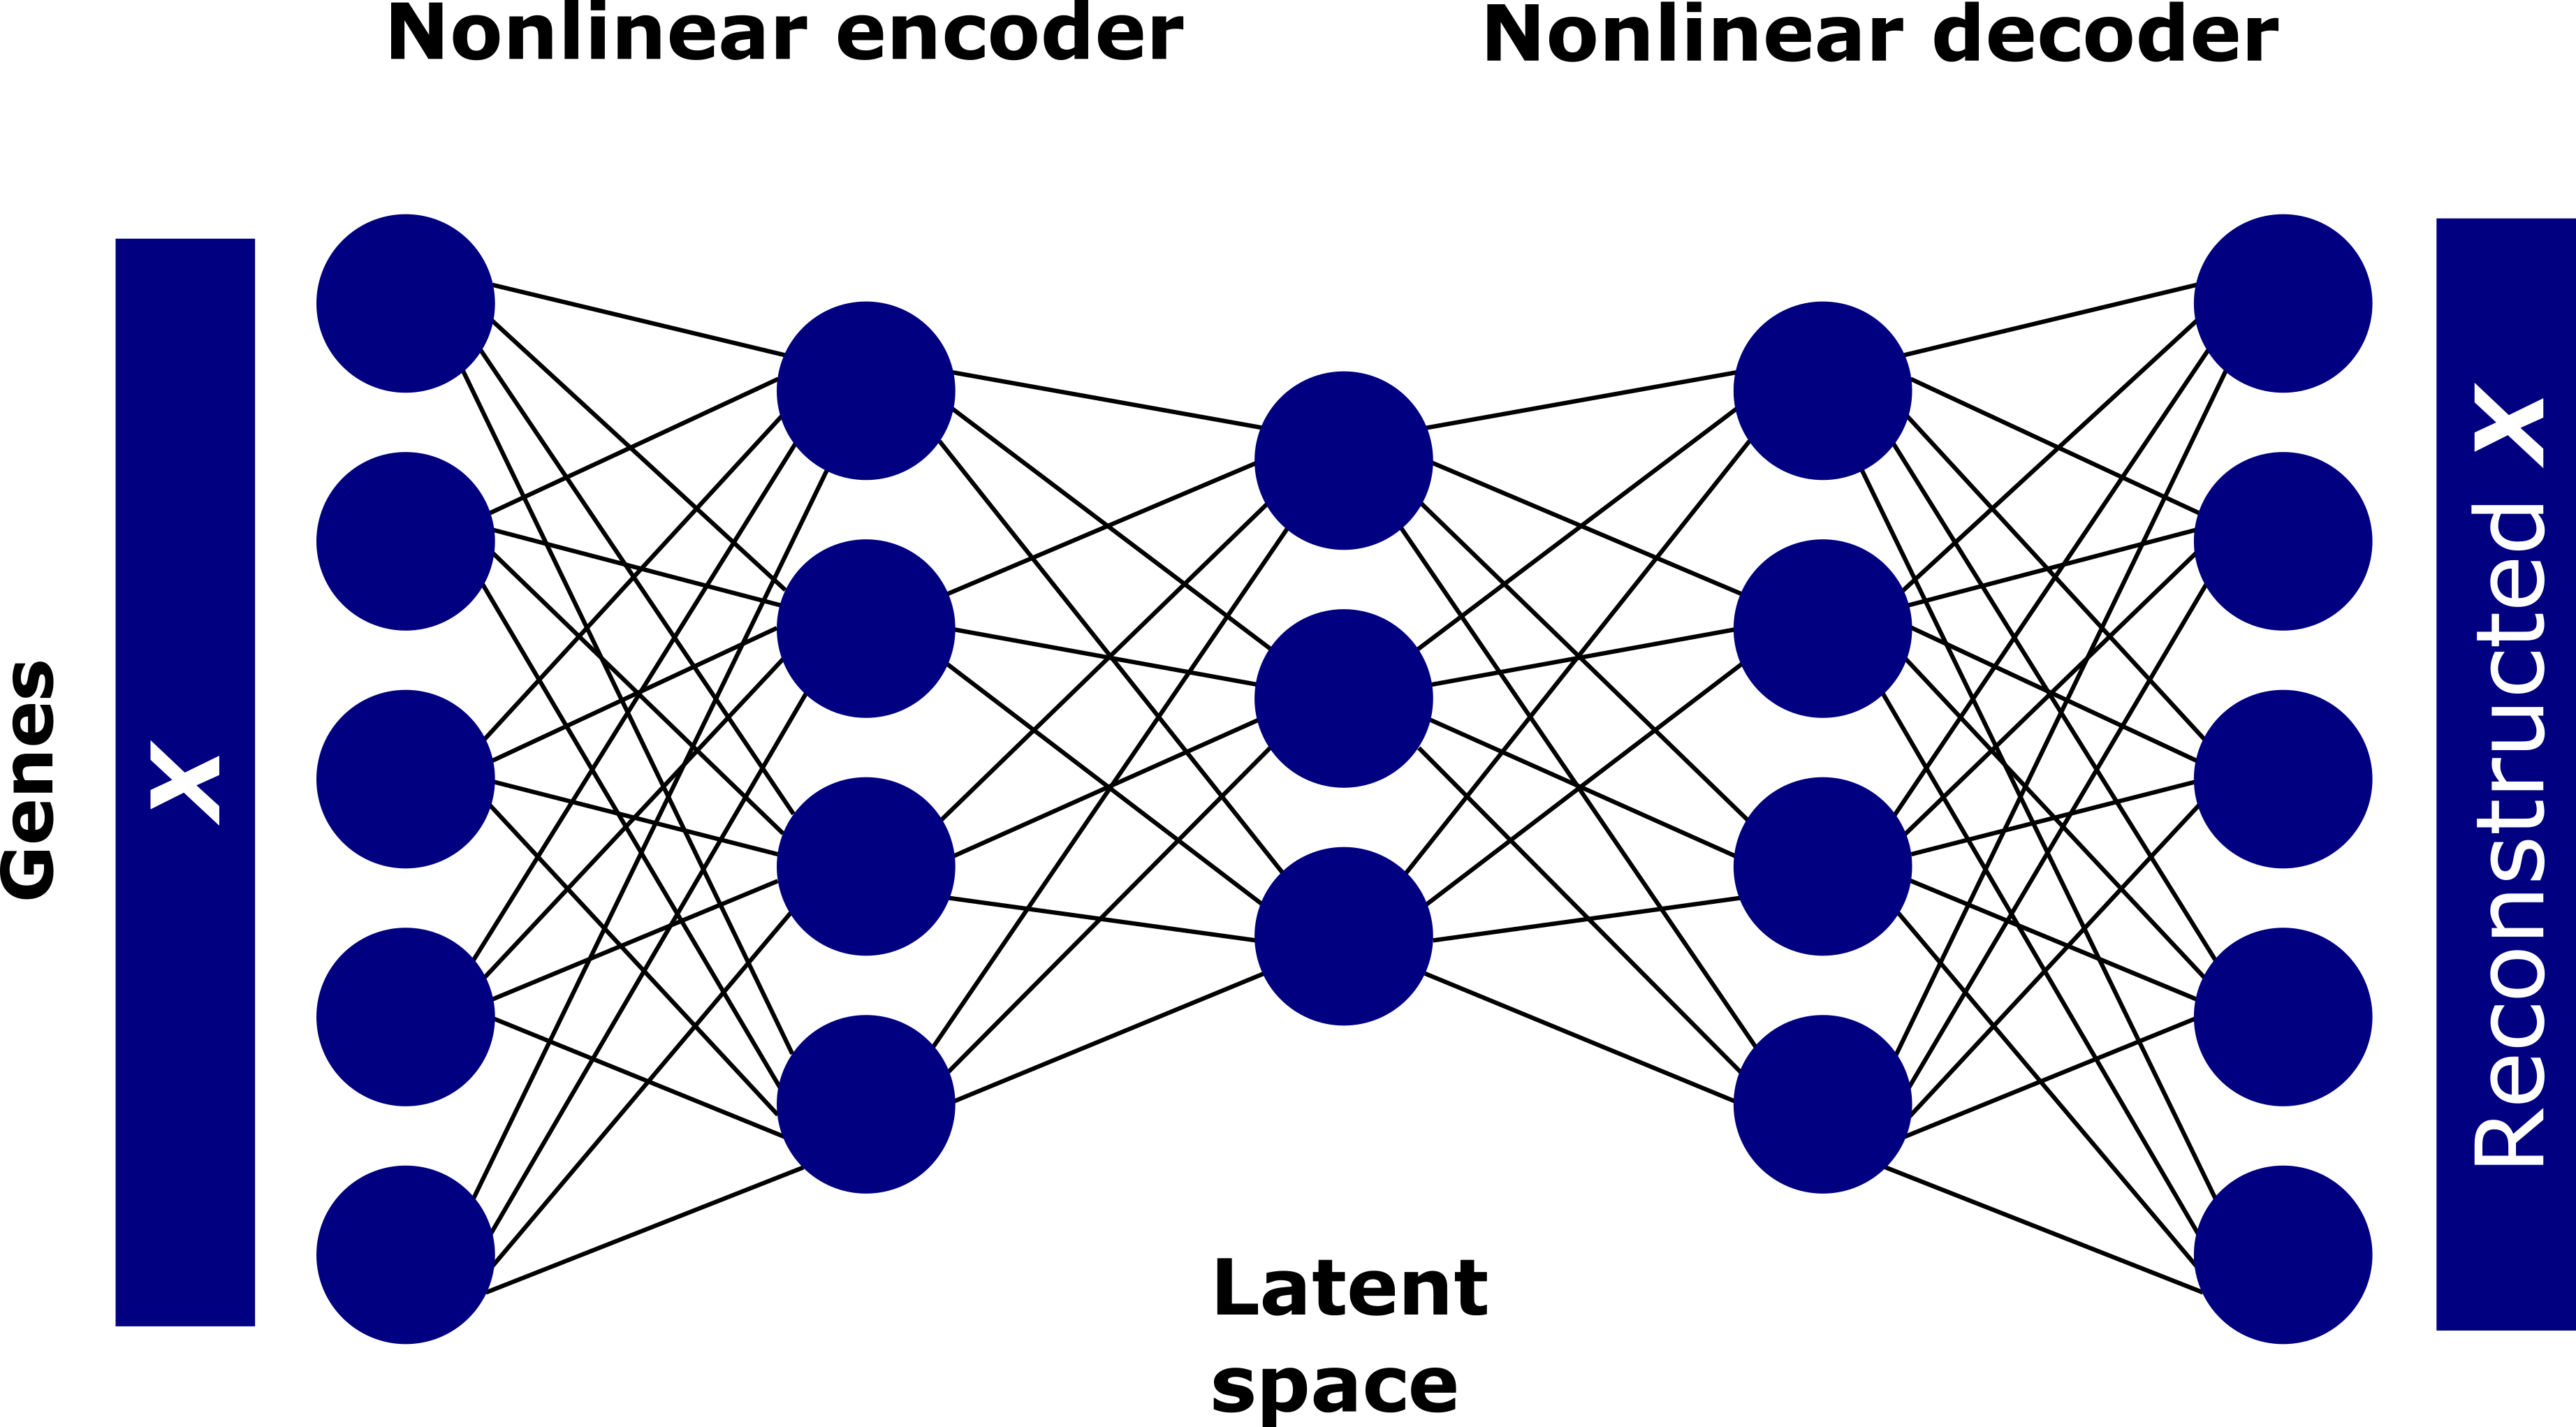
\includegraphics[scale=0.60]{introduction/AE.png}
    \caption{\small{\textbf{Architecture of typical AE}}}
    \label{fig:graphical_abstract_AE}
\end{figure}

\begin{figure}[h!]
    \centering
    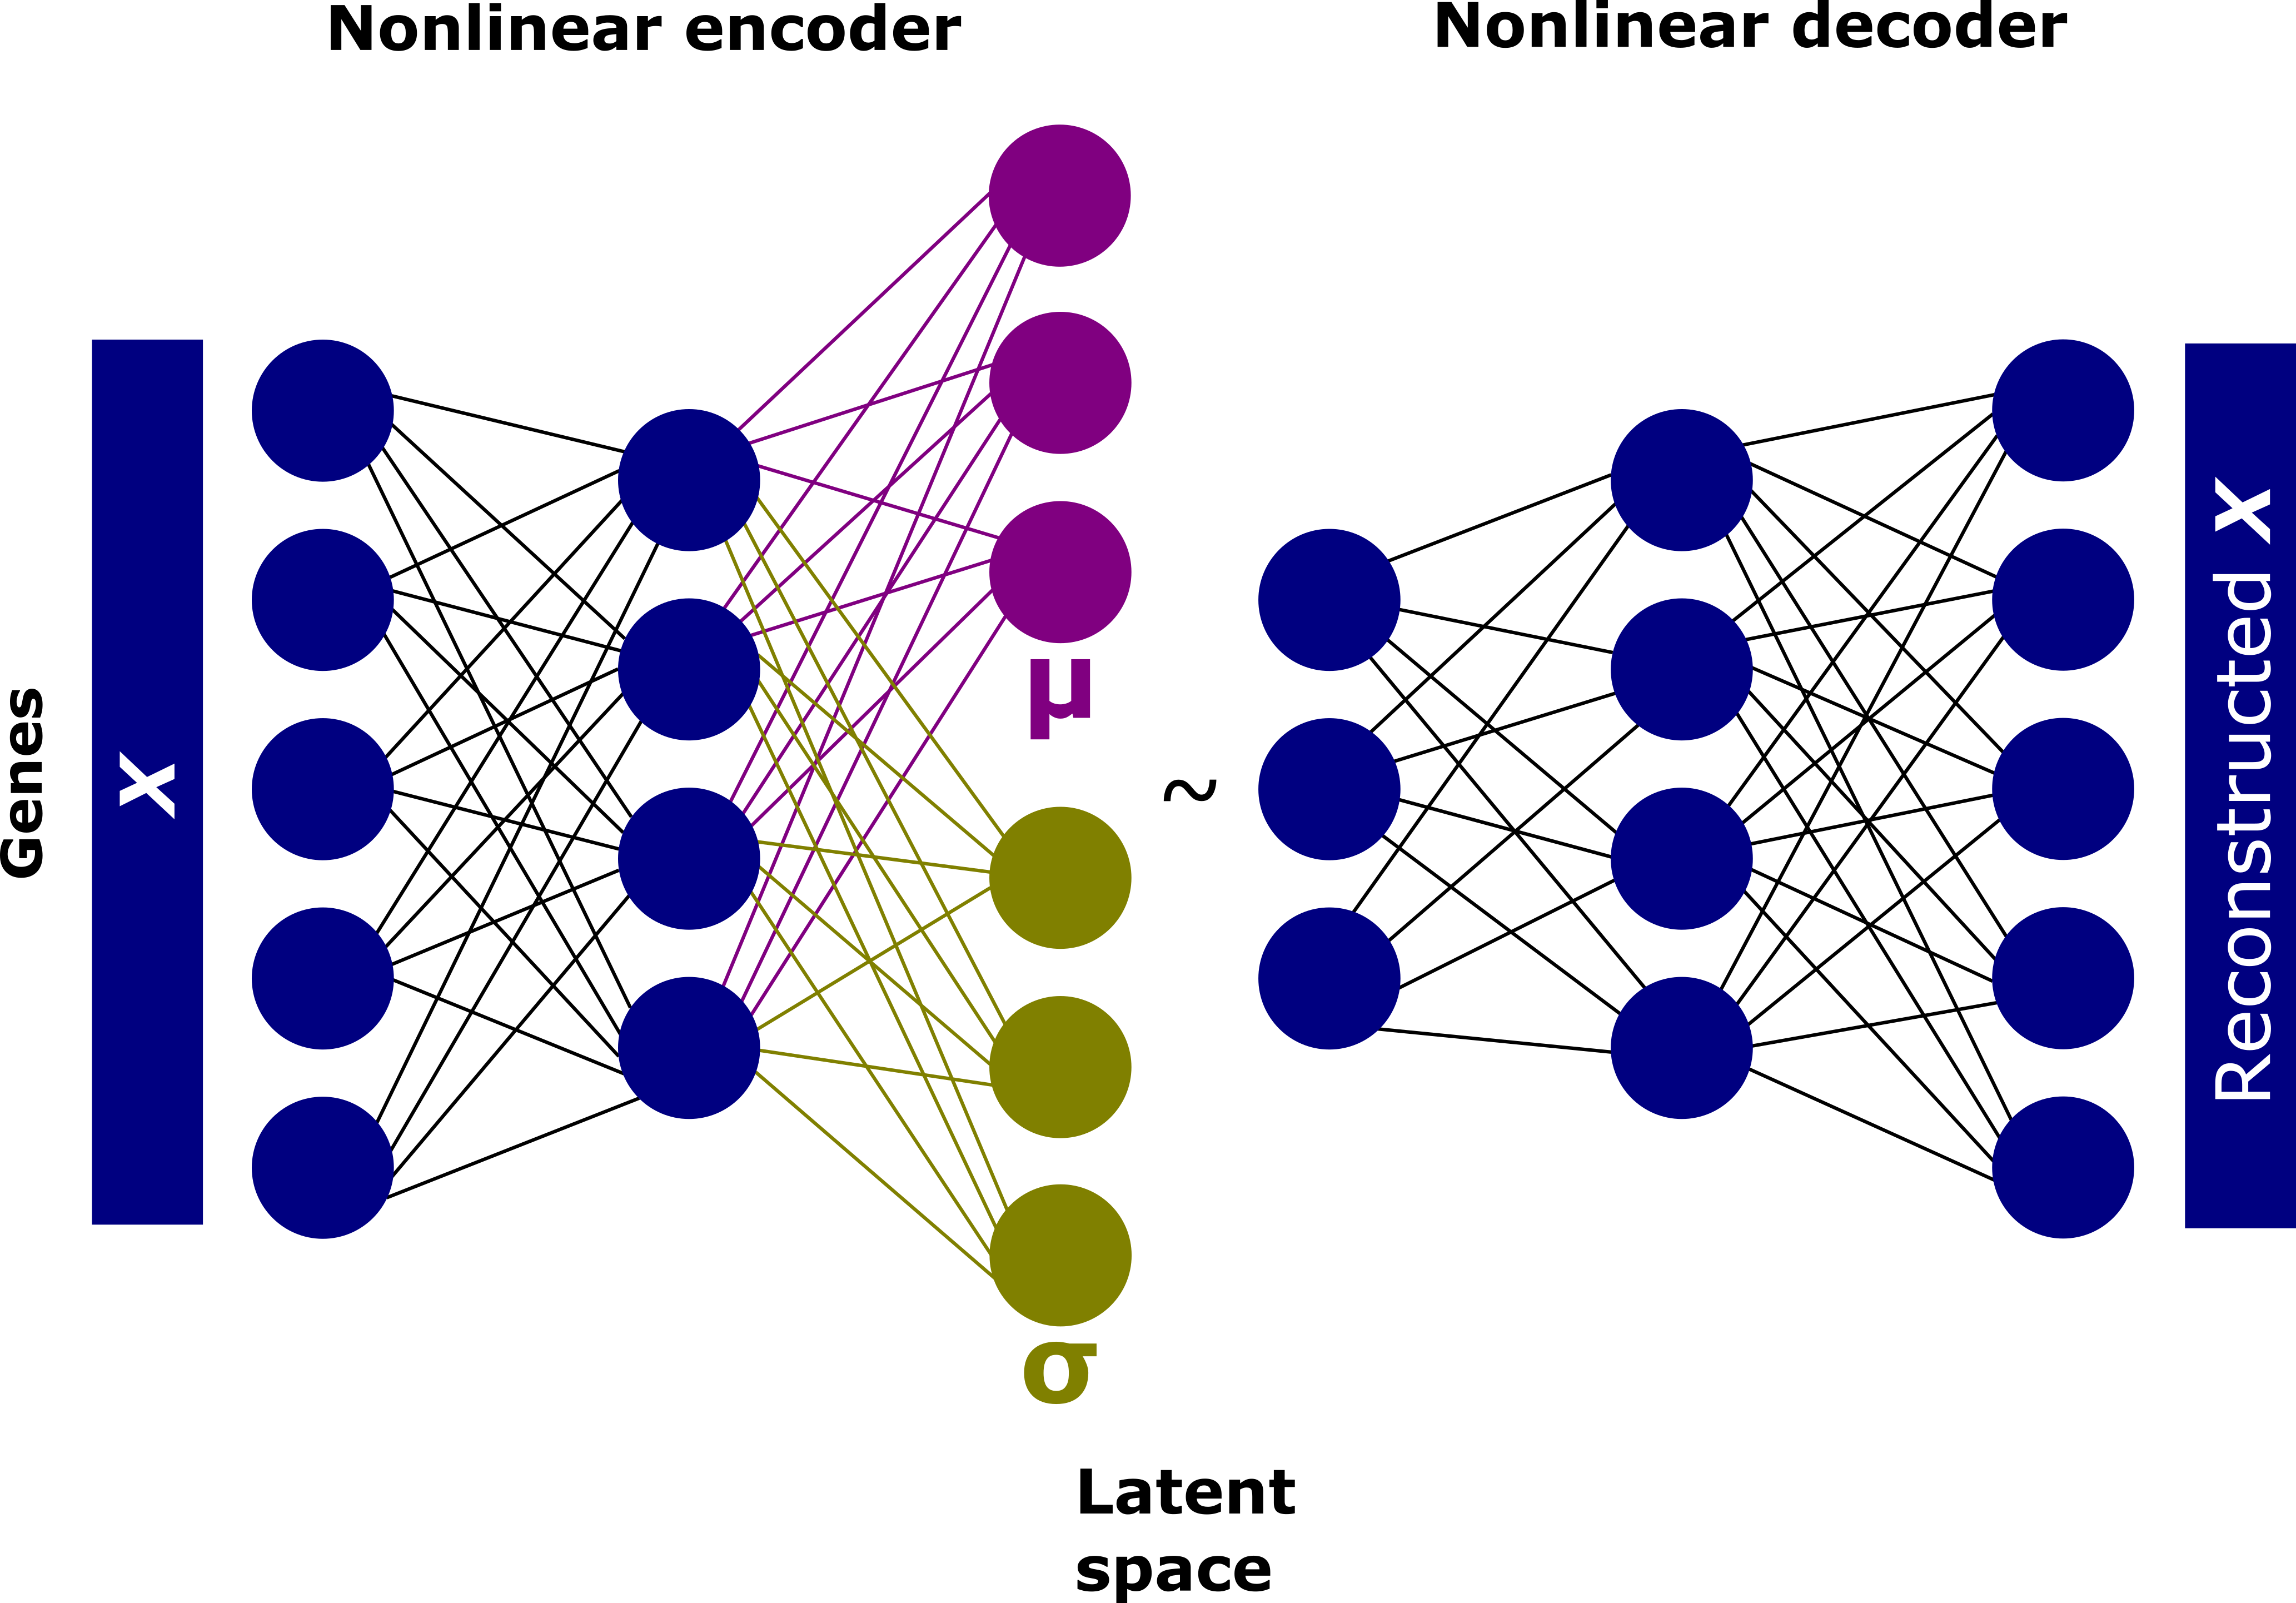
\includegraphics[scale=0.60]{introduction/VAE.png}
    \caption{\small{\textbf{Architecture of typical VAE}}}
    \label{fig:graphical_abstract_VAE}
\end{figure}

\section{Interpretable variational autoencoders}\label{introduction:model}
Inspired by f-scLVM\cite{Buettner2017} that uses prior gene set annotations to guide factor analysis and VAEs which use a factor model as a decoder\cite{Svensson2020}, a novel network architecture called VEGA (VAE enhanced by gene annotations) was proposed by Seninge et al. (2021), which consists of a two-layer nonlinear encoder and a single-layer masked linear decoder (Fig.\ref{fig:graphical_abstract}). Owing to the single-layer decoder where the latent variables (the representation of a single-cell transcriptome) directly connect to the output variables (the gene features), predefined gene set annotations either taken from databases (e.g., Reactome\cite{Gillespie2022} and MSigDB\cite{Liberzon2015}) or inferred using computational methods (e.g., SCENIC\cite{Aibar2017} and ARACNE\cite{Margolin2006}) can be used to guide the decoder wiring through a binary mask, which models the latent variables as biologically meaningful gene modules referred to as gene module variables (GMVs, see Methods \ref{methods:model}). To be more concrete, the values of gene expression of each cell are input to the encoder and encoded to the certain number of latent variables depending on the number of predefined gene modules provided. With the single-layer decoder, the connections between each latent variable and the genes in the output layer can be initiated by the prior gene set annotations, forcing the latent variables to be meaningful and interpretable by limiting them to certain corresponding sets of genes. Since any biological processes can be related to genes, it makes VEGA extremely flexible in terms of the specification of the connectivity of GMVs, which enables us to interpret single-cell transcriptomes from many other different viewpoints. Furthermore, since the decoder was designed as a linear factor model, the weights of a certain GMV to the gene reconstructions can be directly interpreted as the relationships between the GMV and the genes. Last, because different single-cell sequencing measurements always have technical noise and bias, VEGA can also incorporate batch information into the encoder and the latent space through one-hot encoding to combat batch effects, which was introduced in Lopez et al. (2018). Nevertheless, VEGA's hard-coded linear decoder leaves no room for further correcting or expanding existing prior knowledge which is usually incomplete or non-context-specific\cite{Seninge2021}. To have the decoder use prior knowledge more flexibly, instead of hard coding the decoder wiring, the L1 regularization technique\cite{Ng2004} can be employed on weights in the decoder to penalize those unannotated connections, which was introduced in Rybakov et al.(2020). Oppositely to the description above, predefined gene modules are used to pinpoint those GMV-gene relationships which are not included in the prior and the weights of those decoder connections will be penalized by gradually shrinking them to zero (see Methods \ref{methods:L1}). Using the regularized decoder enables the VAE to not only form the interpretable latent space but also potentially recover missing relationships between GMVs and genes in a data-driven fashion.\vspace{2mm}

\begin{figure}[h!]
    \centering
    \hspace*{-4.5mm}
    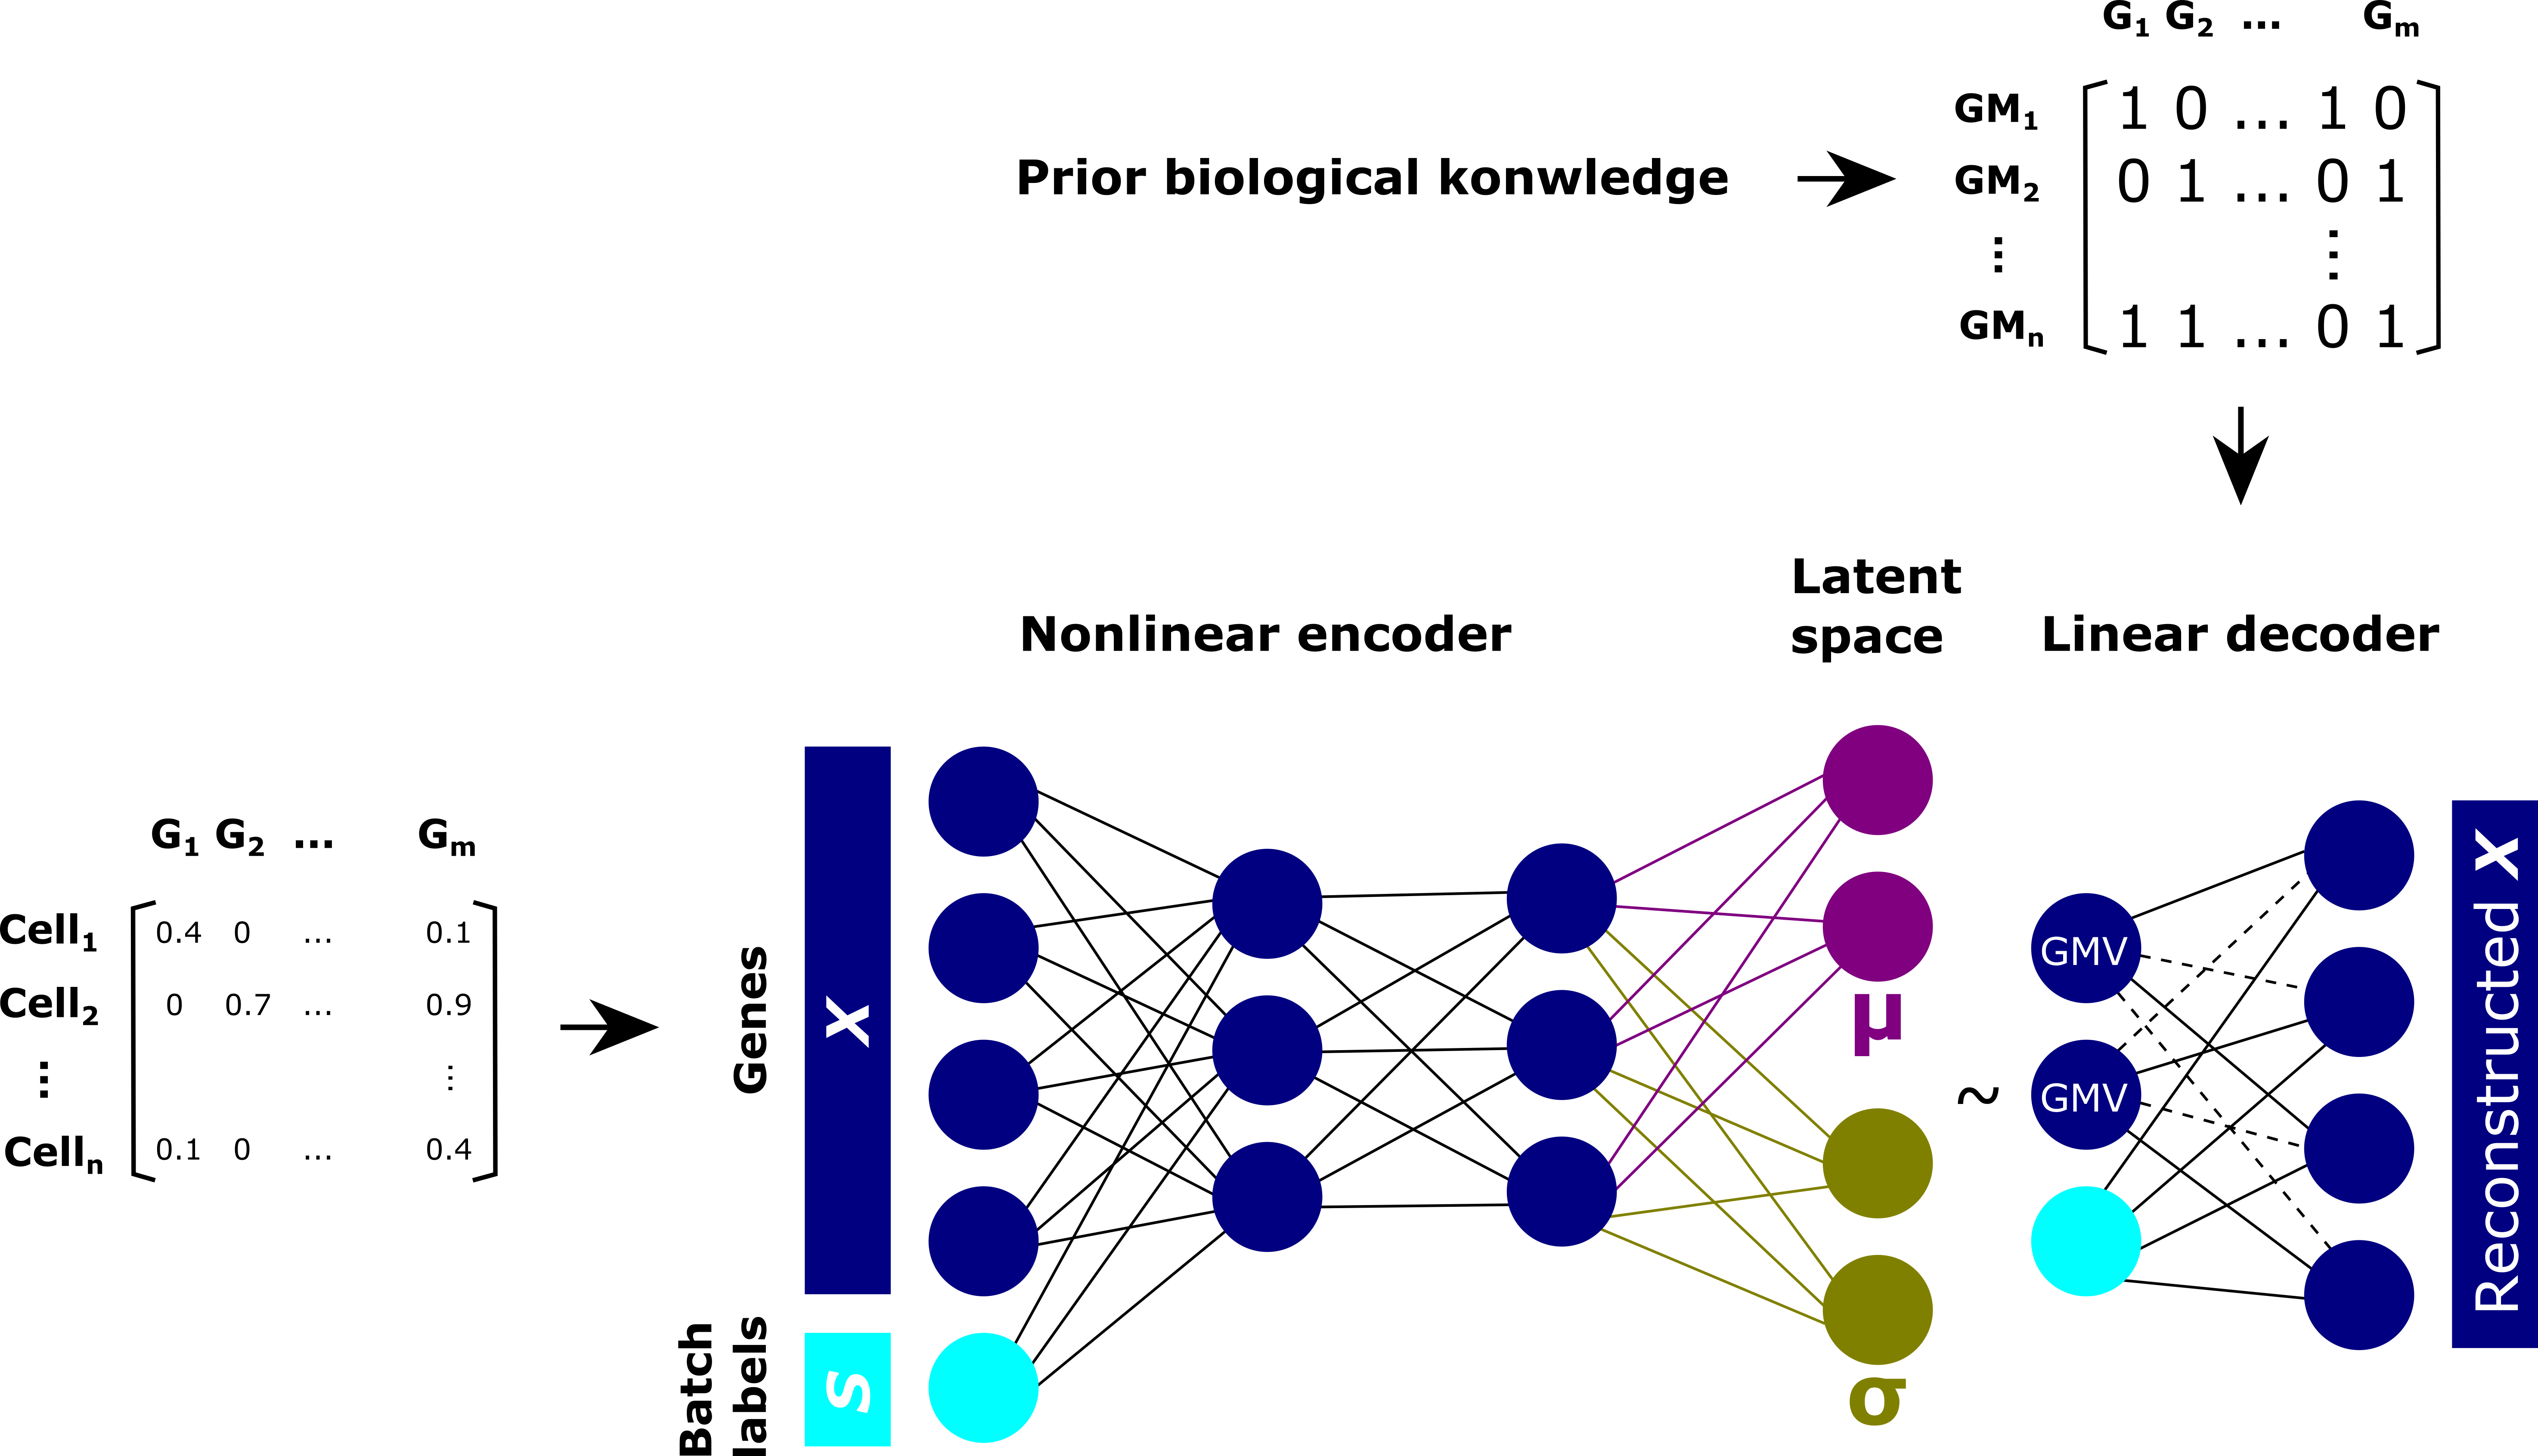
\includegraphics[scale=0.60]{graphical_abstract.png}
    \caption{\small{\textbf{Architecture of interpretable VAE} | The encoder is a two-layer nonlinear neural network which encodes high-dimensional input data to lower-dimensional representations and the representations are then modeled as a multivariate normal distributions in the latent space. The decoder is a single-layer factor model which attempts to reconstruct the representations sampled from the latent normal distribution to the original high-dimensional data. The connections between the latent variables (a representation of input data) and the output variables (input features) can be guided by prior knowledge through a binary mask. For scRNA-seq data analysis, the transcriptome of individual cells is the input to the model and predefined gene modules can be used to guide the decoder wiring. The solid lines in the decoder indicate there are relationships between GMVs and genes according to the prior used and the dashed lines indicate the opposite. There are two circumstances: (1) for the hard-coded decoder, the dashed connections always have zero-valued weights and (2) for the regularized decoder, the weights of the dashed connections are penalized through gradually shrinking them to zero. Moreover, batch information can also be incorporated into the encoder and the latent space through one-hot encoding to alleviate batch effects if needed. G above the matrices stands for gene and GM beside the binary matrix stands for gene module. GMVs represent gene module variables in the latent space.}}
    \label{fig:graphical_abstract}
\end{figure}

\section{Outline of our work}
In this work, we aimed at investigating the ability and various properties of interpretable VAEs that use the hard-coded decoder\cite{Seninge2021} and use the regularized decoder\cite{Rybakov2020}. Our work can be roughly split into three parts; firstly, to verify the availability of VEGA and better understand how exactly the model works, we reproduced the analyses of the well-studied PBMCs (peripheral blood mononuclear cells) dataset\cite{Kang2018} in the VEGA paper\cite{Seninge2021} using the Reactome pathways\cite{Jassal2020} as prior knowledge. Moreover, we sought to improve the model reproducibility which is important to the VEGA's main characteristic, interpretability, so we explored potential ways to boost the model reproducibility using the same dataset and prior knowledge. Secondly, we performed the benchmark studies on VEGA using the published human adrenal medulla dataset\cite{Jansky2021} and the SCENIC regulons\cite{Jansky2021} inferred from the same dataset as the prior. Note that we took advantage of the inferred TF activities of each adrenal medulla cell type group described in Jansky et al. (2021) as references for our benchmarks. Furthermore, we also employed the non-context-specific DoRothEA regulons\cite{Garcia-Alonso2019} as prior knowledge to observe the changes in the behavior of VEGA. Inspired by the results from the analyses of the adrenal medulla dataset\cite{Jansky2021} using the DoRothEA regulons as the prior, we investigated the tolerance of VEGA to incorrect information in prior knowledge by randomizing prior gene set annotations to different degrees. The last task we conducted in this section was testing the batch correction function\cite{Lopez2018} that is incorporated in VEGA. To do so, we took advantage of the human neuroblastoma dataset\cite{Jansky2021} which consists of 22 neuroblastoma samples and suffers from severe batch effects and the SCENIC regulons inferred from this tumor data as prior knowledge to see if VEGA is capable of screening out technical differences. In the last part of our work, we investigated the behavior and the ability of the interpretable VAE model using the regularized decoder by artificially modifying prior gene set annotations (i.e., artificial gene removal and addition) to see whether the regularized decoder manages to recover missing target genes or exclude non-biologically meaningful genes. Last, we studied the inference capacity of the regularized decoder by using the non-context-specific DoRothEA regulons as the prior, that is, we were interested in if the regularized decoder can infer more dataset-specific GRNs from general GRNs.
